\chapter{BIPEDAL WALKING BY TWIN DELAYED DEEP DETERMINISTIC POLICY GRADIENTS}
\label{chap:exp_setup}

\section{Details of the Environment}

\textit{BipedalWalker-v3} and \textit{BipedalWalker-Hardocore-v3} are simulation environments of a bipedal robot, 
with relatively flat course and obstacle course respectively. 
Dynamics of the robot are exactly identical in both environments. 
Our task is to solve hardcore version where the agent is expected to learn to run and walk in different road conditions. 
Components of the hardcore environment is visualized in \figref{fig:bipedal_hardcore_components}. 

\begin{figure}
	\centering
	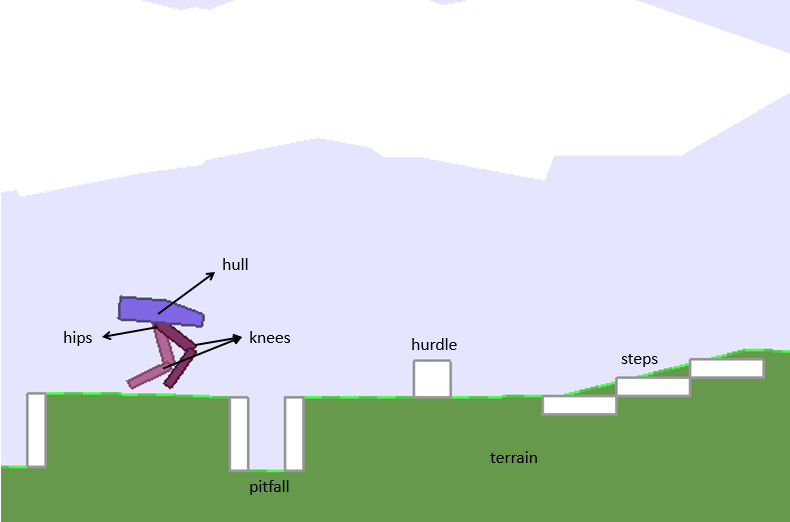
\includegraphics[width=0.95\textwidth]{figures/bipedal/bpedal_annotated.png}
	\caption{Bipedal Walker Hardcore Components}
	\label{fig:bipedal_hardcore_components}
\end{figure}

The robot has kinematic and lidar sensors. 
It is modeled as Markov Decision Process with deterministic dynamics. 

\textbf{Observation Space} contains hull angle, hull angular velocity, hull translational velocities, joint positions, joint angular speeds, leg ground concats and 10 lidar rangefinder measurements. Details are summarized at Table \tabref{table:bpw_obs_space}. 

\begin{table}%[h!]
	\begin{center}
	\begin{tabular}{cccc}
		\textbf{Num} & \textbf{Observation} & \textbf{Interval} \\
		\hline 
		0  & Hull Angle & $[-\pi,\pi]$ \\
		1  & Hull Angular Speed & $[-\infty,\infty]$ \\
		2  & Hull Horizontal Speed x & $[-1,1]$ \\
		3  & Hull Vertical Speed &$[-1,1]$ \\
		4  & Hip 1 Joint Angle & $[-\infty,\infty]$ \\
		5  & Hip 1 Joint Speed & $[-\infty,\infty]$ \\
		6  & Knee 1 Joint Angle & $[-\infty,\infty]$ \\
		7  & Knee 1 Joint Speed & $[-\infty,\infty]$ \\
		8  & Leg 1 Ground Contact Flag & $\{0,1\}$ \\
		9  & Hip 2 Joint Angle & $[-\infty,\infty]$ \\
		10  & Hip 2 Joint Speed & $[-\infty,\infty]$ \\
		11  & Knee 2 Joint Angle & $[-\infty,\infty]$ \\
		12  & Knee 2 Joint Speed & $[-\infty,\infty]$ \\
		13  & Leg 2 Ground Contact Flag & $\{0,1\}$ \\
		14-23  & Lidar measures  & $[-\infty,\infty]$
	\end{tabular}
	\end{center}
	\caption{Observation Space of Bipedal Walker}
	\label{table:bpw_obs_space}
\end{table}

The robot has 2 legs with 2 joints at knee and hip. Torque provided to knee and pelvis joints of both legs. These 4 torque values forms  \textbf{Action Space}. Details are presented in \tabref{table:bpw_act_space}. 

\begin{table}%[h!]
	\begin{center}
		\begin{tabular}{cccc}
			\textbf{Num} & \textbf{Observation} & \textbf{Interval} \\
			\hline
			0  & Hip 1 Torque & $[-1,1]$ \\
			1  & Hip 2 Torque & $[-1,1]$ \\
			2  & Knee 1 Torque & $[-1,1]$ \\
			3  & Knee 2 Torque & $[-1,1]$ \\
		\end{tabular}
	\end{center}
	\caption{Action Space of Bipedal Walker}
	\label{table:bpw_act_space}
\end{table}

\textbf{Reward Function} is a bit complex. 
The robot should run fast with little energy while should not stumble and fall to ground. 
Therefore reward is shaped accordingly. 
Directly proportional to distance traveled forward, +300 points given if agent reaches end of path. 
-10 points (-100 points in original version) if agent falls, 
and small amount of negative reward proportional to applied motor torque (to prevent applying unnecessary torque). 
Lastly, the robots gets negative reward propotional to absolut value of hull angle for reinforcing to keep hull straigth. 

\subsection{Partial Observability}

The environment is partially observable due to following reasons.
\begin{itemize}
	\item The agent is not able to track behind with lidar sensor. 
	Unless it has a memory, it cannot know whether a pitfall or hurdle behind. 
	Illustration is shown in \figref{fig:partial_obs_pitfall}.
	\item There is no accelerometer sensor. 
	Therefore, the agent do not know whether it is accelerating or decelerating.
\end{itemize}

\begin{figure}
	\begin{subfigure}{.32\textwidth}
		\centering
		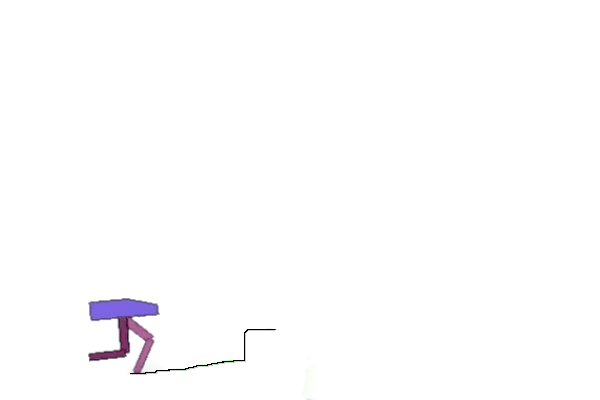
\includegraphics[width=0.99\linewidth]{figures/bipedal/po/lidarcover.png}
		\caption{Perspective}
		\label{fig:lidar_cover}
	\end{subfigure}
	\begin{subfigure}{.32\textwidth}
		\centering
		
\includegraphics[width=0.99\linewidth]{figures/bipedal/po/pitfall_behind.png}
		\caption{Pitfall Behind}
		\label{fig:pitfall_behind}
	\end{subfigure}
		\begin{subfigure}{.32\textwidth}
		\centering
		
\includegraphics[width=0.99\linewidth]{figures/bipedal/po/no_pitfall_behind.png}
		\caption{No Pitfall Behind}
		\label{fig:no_pitfall_behind}
	\end{subfigure}
	\caption{Perspective of agent and possible realities}
	\label{fig:partial_obs_pitfall}
\end{figure}

In DRL, partial observability is handled by 2 ways in literature~ \cite{dulac-arnold_challenges_2019}. 
First is incorprating fixed number of last observations while second way is updating hidden belief state using recurrent neural network at each time step. 
Our approach is using fixed number of past observation into LSTM and Transformer based networks for both actor and critic networks. 

\subsection{Reward Sparsity}

Rewards given to the agent is sparse in some circumstances. 
\begin{itemize}
	\item Overcoming big hurdles requires a very specific move. 
	The agent should explore many actions when faced with a big hurdle.
	\item Crossing pitfalls also require a specific move but not as complex as big hurdles.
\end{itemize}

\subsection{Modifications on Original Envrionment}

It is difficult to solve directly available environment as it is. 
Therefore, there are few works on the literature demonstrating a solution. 
\begin{itemize}
	\item In original version, agent gets -100 points when its hull hits the floor. 
	In order to make the robot more greedy, this is changed to -10 points. 
	Otherwise, agent cannot explore environment since it gets too much punisment when failed.
	\item Time frequency of simulation is halved (from 50 Hz to 25 Hz) by only observing last of each two consecutive frames using a custom wrapper function. 
	Since there is not a high frequency dynamics, this allows nothing but speeding up the learning process.
	\item In original implementation, an episode has time limit. 
	Once this limit is reached, simulation stops with terminal flag. 
	On the other hand, when agent fails before time limit, the episode ends with terminal flag too. 
	In first case, the terminal flag causes instability since next step's value is not used in value update. 
	The environment changed such that terminal flag is not given in this case unless agent fails.
\end{itemize}


